% ---
% Reemplaza líneas 3458–3462 de Docs/Technical_Report.tex.
% Decisiones y hallazgos que lo respaldan: D-039, D-040, H-049, H-050.
% ---

\subsection{Evaluación comparativa}

% fuente: H-049; 8_spearman.csv, 8_rangos.csv
% Generado por Code/tools/tablas_latex.py desde 8_spearman.csv. No editar a mano: volver a correr el script.
\begin{table}[H]
\centering
\small
\caption{Correlación de Spearman entre el orden de separabilidad y el de clasificación de las cinco condiciones (M8).}
\label{tab:m8_spearman}
\begin{adjustbox}{max width=\linewidth}
\begin{tabular}{l l r r}
\toprule
Subconjunto & Métrica de separabilidad & $\rho_s$ & $p$ exacto bilateral \\
\midrule
Masas & Davies--Bouldin & 0.718 & 0.167 \\
Masas & Fisher $J$ & \textbf{0.821} & 0.133 \\
Masas & KTA lineal & 0.718 & 0.167 \\
Calcificaciones & Davies--Bouldin & \textbf{0.975} & 0.033 \\
Calcificaciones & Fisher $J$ & 0.667 & 0.267 \\
Calcificaciones & KTA lineal & \textbf{0.975} & 0.033 \\
\bottomrule
\end{tabular}
\end{adjustbox}
\par\smallskip
\parbox{0.95\linewidth}{\footnotesize Submuestra de 200 lesiones frente al AUC de prueba, $k = 12$. Con $n = 5$ hay 120 órdenes; $\rho_s$ es la correlación de Pearson de los rangos promedio, porque C1 y C2 empatan. Es descriptivo: con el empate, el mejor orden alcanzable da $p = 4/120$. En negritas, la métrica con mayor $\rho_s$ en cada subconjunto.}
\end{table}


% fuente: H-049; 8_spearman.csv, 8_rangos.csv, 8_spearman_nula.csv
La correlación de rangos de Spearman ($\rho_s$) entre los ordenamientos de separabilidad espacial calculados en el espacio de \textit{embedding} y el orden de desempeño clasificatorio en el conjunto de prueba se presenta en el cuadro~\ref{tab:m8_spearman}. Conforme al diseño metodológico, dicho coeficiente se evalúa de manera descriptiva: para $n = 5$ condiciones existen únicamente $5! = 120$ permutaciones posibles, y dado que las condiciones clásicas C1 y C2 empatan de forma exacta en toda métrica geométrica afín por construcción, el valor máximo teóricamente alcanzable es $\rho_s = 0.975$, cuya probabilidad nula exacta bilateral es $p = 4/120 \approx 0.033$. En la muestra primaria de 200 lesiones a $k = 12$, los coeficientes observados son positivos en su totalidad: en masas, el índice de Davies--Bouldin arroja $\rho_s = 0.718$ ($p = 0.167$), la razón de Fisher $J$ obtiene $\rho_s = 0.821$ ($p = 0.133$) y la alineación KTA lineal registra $\rho_s = 0.718$ ($p = 0.167$); en calcificaciones, Davies--Bouldin y KTA lineal alcanzan el acuerdo máximo posible con $\rho_s = 0.975$ ($p = 0.033$), mientras que Fisher $J$ registra $\rho_s = 0.667$ ($p = 0.267$).

% fuente: H-049; 8_spearman.csv, 8_rangos.csv
Al considerar el análisis de sensibilidad exhaustivo sobre los 48 coeficientes de correlación calculados (combinando tres métricas de separabilidad, dos tamaños de muestra, dos evaluaciones de clasificación y los valores $k \in \{8, 12\}$), la totalidad de los valores se mantiene estrictamente positiva en el rango de 0.67 a 0.97. En todas las instancias evaluadas, los ordenamientos sitúan sin excepción al bloque de las tres condiciones clásicas (C1, C2 y C3) por delante del bloque de representaciones cuánticas (C4 y C5). Las fluctuaciones menores observadas al interior de cada bloque reflejan ruido numérico propio del entrenamiento. Asimismo, en el espacio de kernels ($n = 3$), el kernel RBF clásico lidera tanto en alineamiento de matrices como en clasificación con SVM respecto a las variantes cuánticas C4 y C5. Estos resultados confirman que las métricas de separabilidad geométrica reflejan adecuadamente la capacidad clasificatoria ulterior, evidenciando de manera coherente la ausencia de beneficio clasificatorio derivado de la transformación cuántica.

\begin{figure}[htbp]
\centering
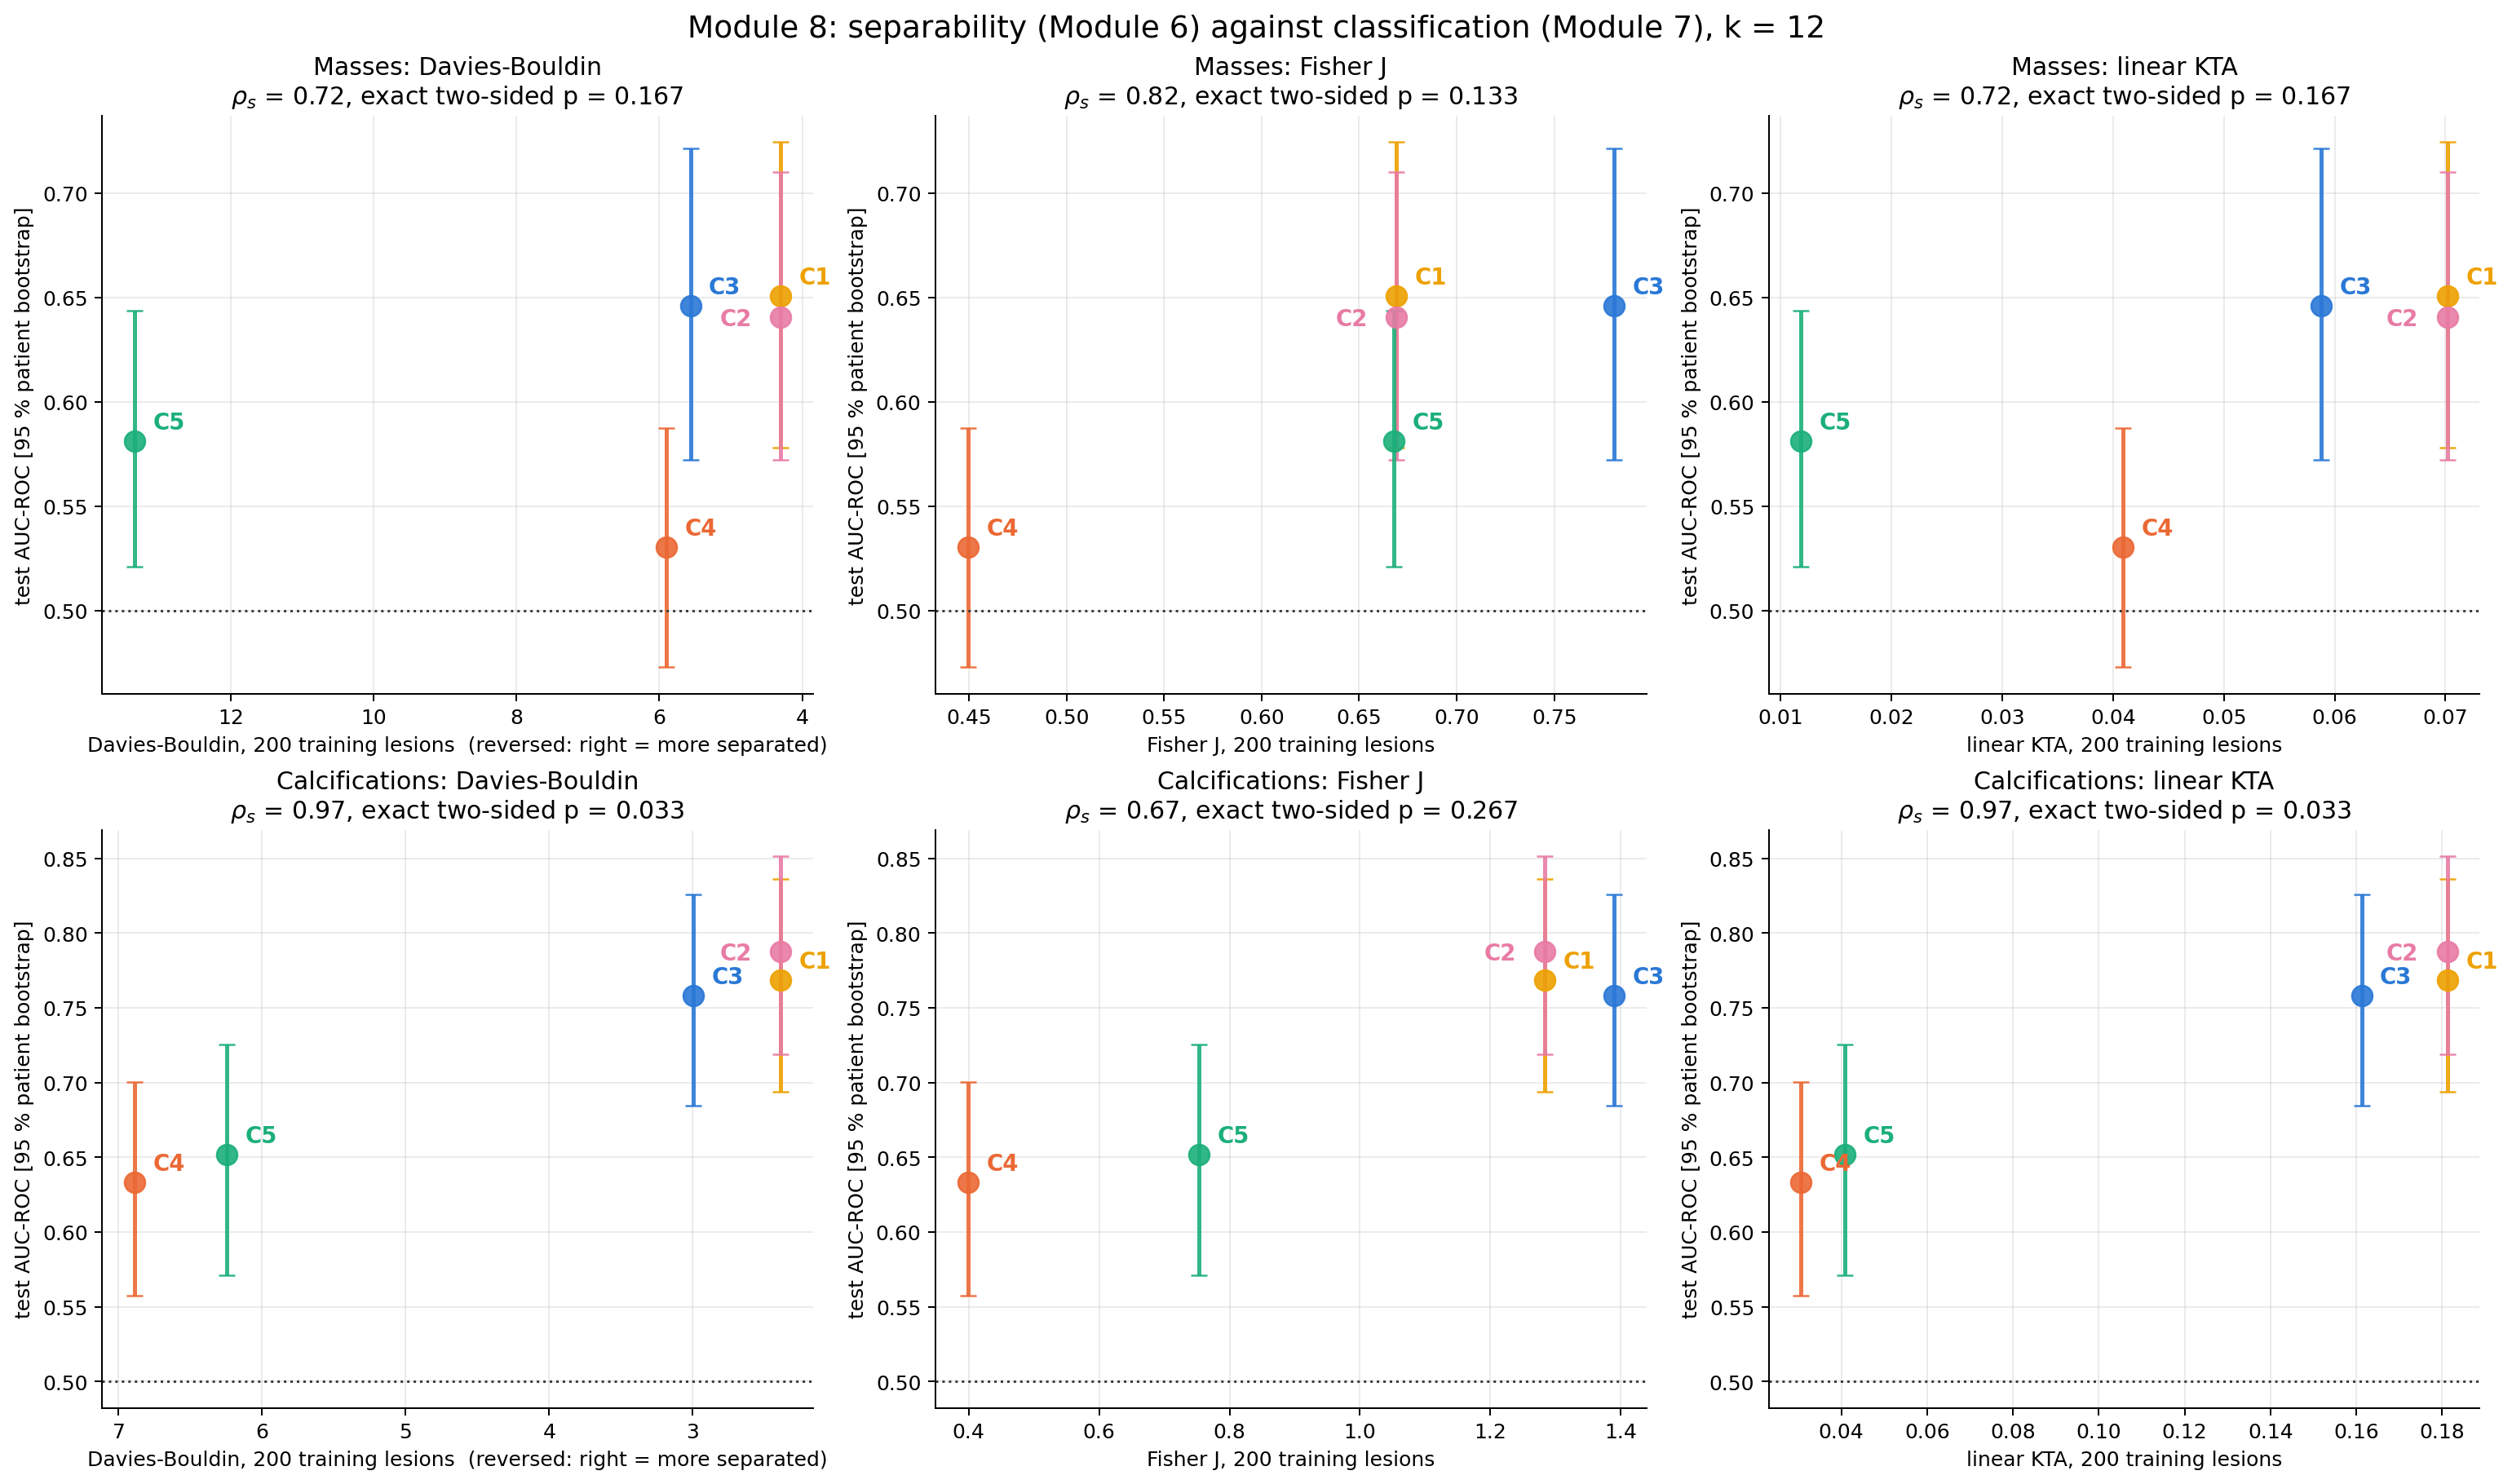
\includegraphics[width=\textwidth]{Figures/M8_spearman.png}
\caption{Correlación de Spearman entre los ordenamientos de separabilidad del espacio de estados y el desempeño de clasificación en el conjunto de prueba oficial.}
\label{fig:m8_spearman}
\end{figure}

\begin{figure}[htbp]
\centering
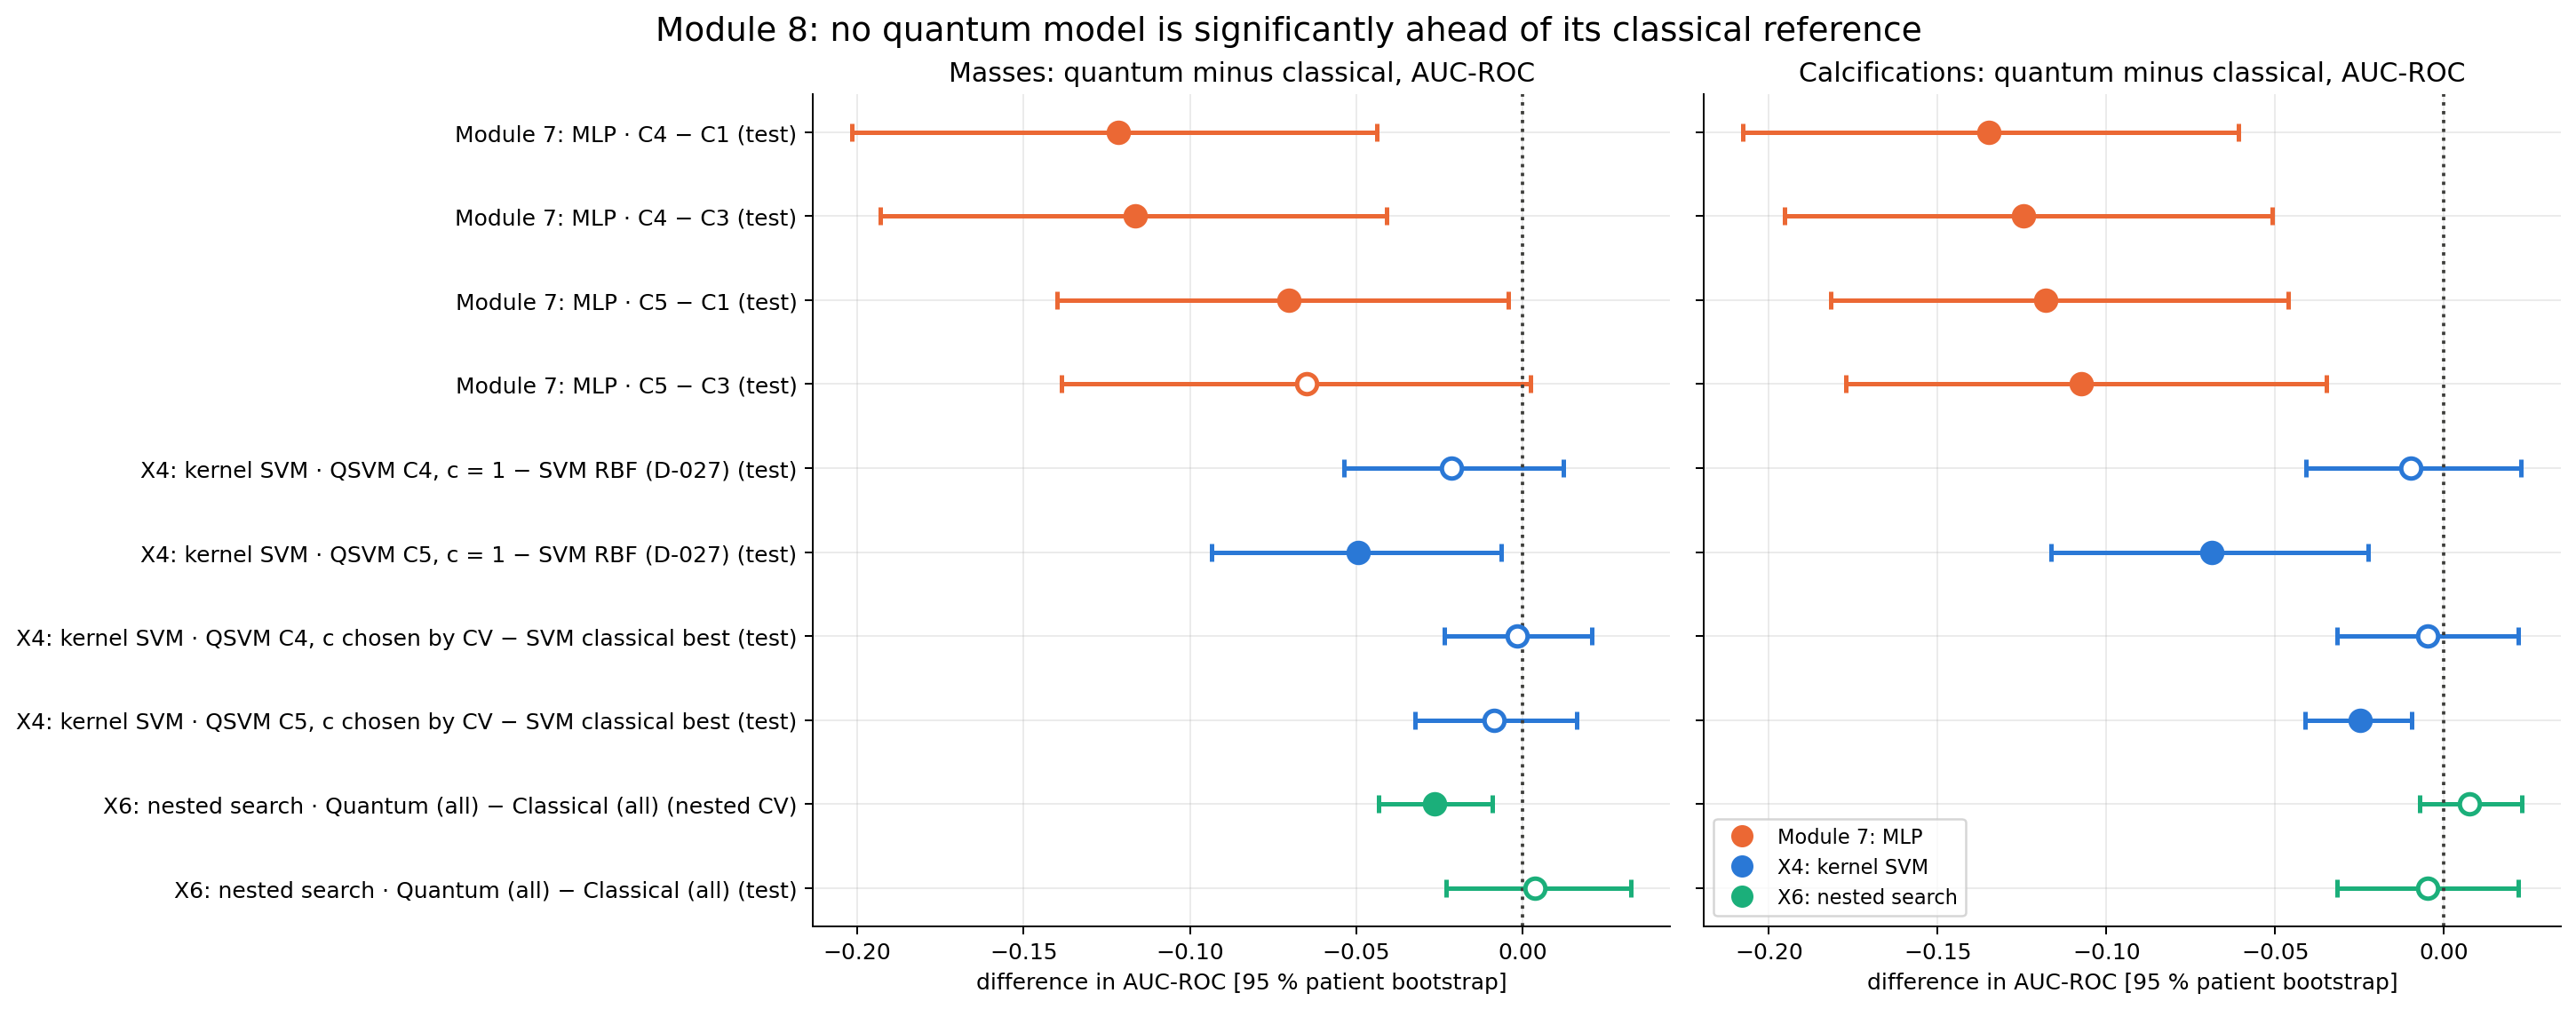
\includegraphics[width=\textwidth]{Figures/M8_classical_vs_quantum.png}
\caption{Dispersión bivariada y contraste pareado de métricas de separabilidad frente al AUC de clasificación entre condiciones clásicas y cuánticas.}
\label{fig:m8_classical_vs_quantum}
\end{figure}

% fuente: H-050; 8_descriptores_radiologo.csv, 8_masas_vs_calcificaciones.csv
La aparente discordancia observada entre el análisis exploratorio inicial ---donde las masas exhibían patrones morfológicos distintivos que sugerían una mayor separabilidad que las calcificaciones--- y el rendimiento del clasificador final se explica por la naturaleza de los descriptores radiómicos extraídos. Al evaluar una regresión logística sobre los descriptores categóricos anotados por el médico radiólogo en CBIS-DDSM (forma y margen en masas; tipo morfológico y distribución en calcificaciones), las masas constituyen el subconjunto más separable, alcanzando un AUC en validación cruzada de 0.872 frente a 0.825 en calcificaciones. Estos descriptores radiológicos operan como una referencia clínica interpretativa y no como un sistema automatizado competidor, dado que fueron asignados mediante inspección médica experta.

% fuente: H-050; 8_descriptores_radiologo.csv, 8_masas_vs_calcificaciones.csv
Al sustituir el juicio experto por las características radiómicas cuantitativas calculadas en el pipeline, el orden de dificultad se invierte: las 67 características radiómicas recuperan un AUC de 0.800 en calcificaciones (muy próximo a los 0.825 del radiólogo), pero descienden a 0.693 en masas (lejos de los 0.872 del radiólogo). Con las 12 características seleccionadas en M4, el AUC se sitúa en 0.745 en calcificaciones y en 0.668 en masas. Esta discrepancia revela que la mayor dificultad clasificatoria en masas es una propiedad de las variables radiómicas cuantitativas estándar empleadas, las cuales resumen la textura y contorno global sin capturar con la misma fidelidad los detalles finos de espiculación perilesional que distingue el ojo experto. Por otra parte, el impacto de la representación cuántica resulta equivalente en ambos subconjuntos: la brecha C4 $-$ C1 es de $-0.12$ en masas y de $-0.14$ en calcificaciones, con medianas del kernel análogas (0.002 a 0.003 en C4; 0.00003 en C5) y diferencias geométricas similares ($g$ entre 1.4 y 1.7), demostrando que la asimetría observada entre patologías obedece a la señal radiómica clásica y no al comportamiento del circuito cuántico.
